\documentclass[a4paper,10pt]{book}\usepackage{graphicx}
\usepackage{epstopdf}
\epstopdfsetup{update} % only regenerate pdf files when eps file is newer
\usepackage[utf8]{inputenc}
\usepackage{graphicx}
\usepackage{hyperref}
\usepackage{float}
\usepackage{tabularx}
\usepackage{pdfpages}

\restylefloat{table}
% Title Page
\title{Exam Report Communication Networks II}
\author{Daniel Plöger, Nina Piontek}

\begin{document}
\maketitle
\tableofcontents



\chapter{Network Description}
Because of a construction site near Channel 4 which might accidentally damage the cables 
used for internet connection,
a point-to-point radio link should be implemented to ensure network connection.
In the following, the new network configuration as depicted in \ref{fig:network} will be evaluated.
\begin{figure}[!ht]
  \centering
    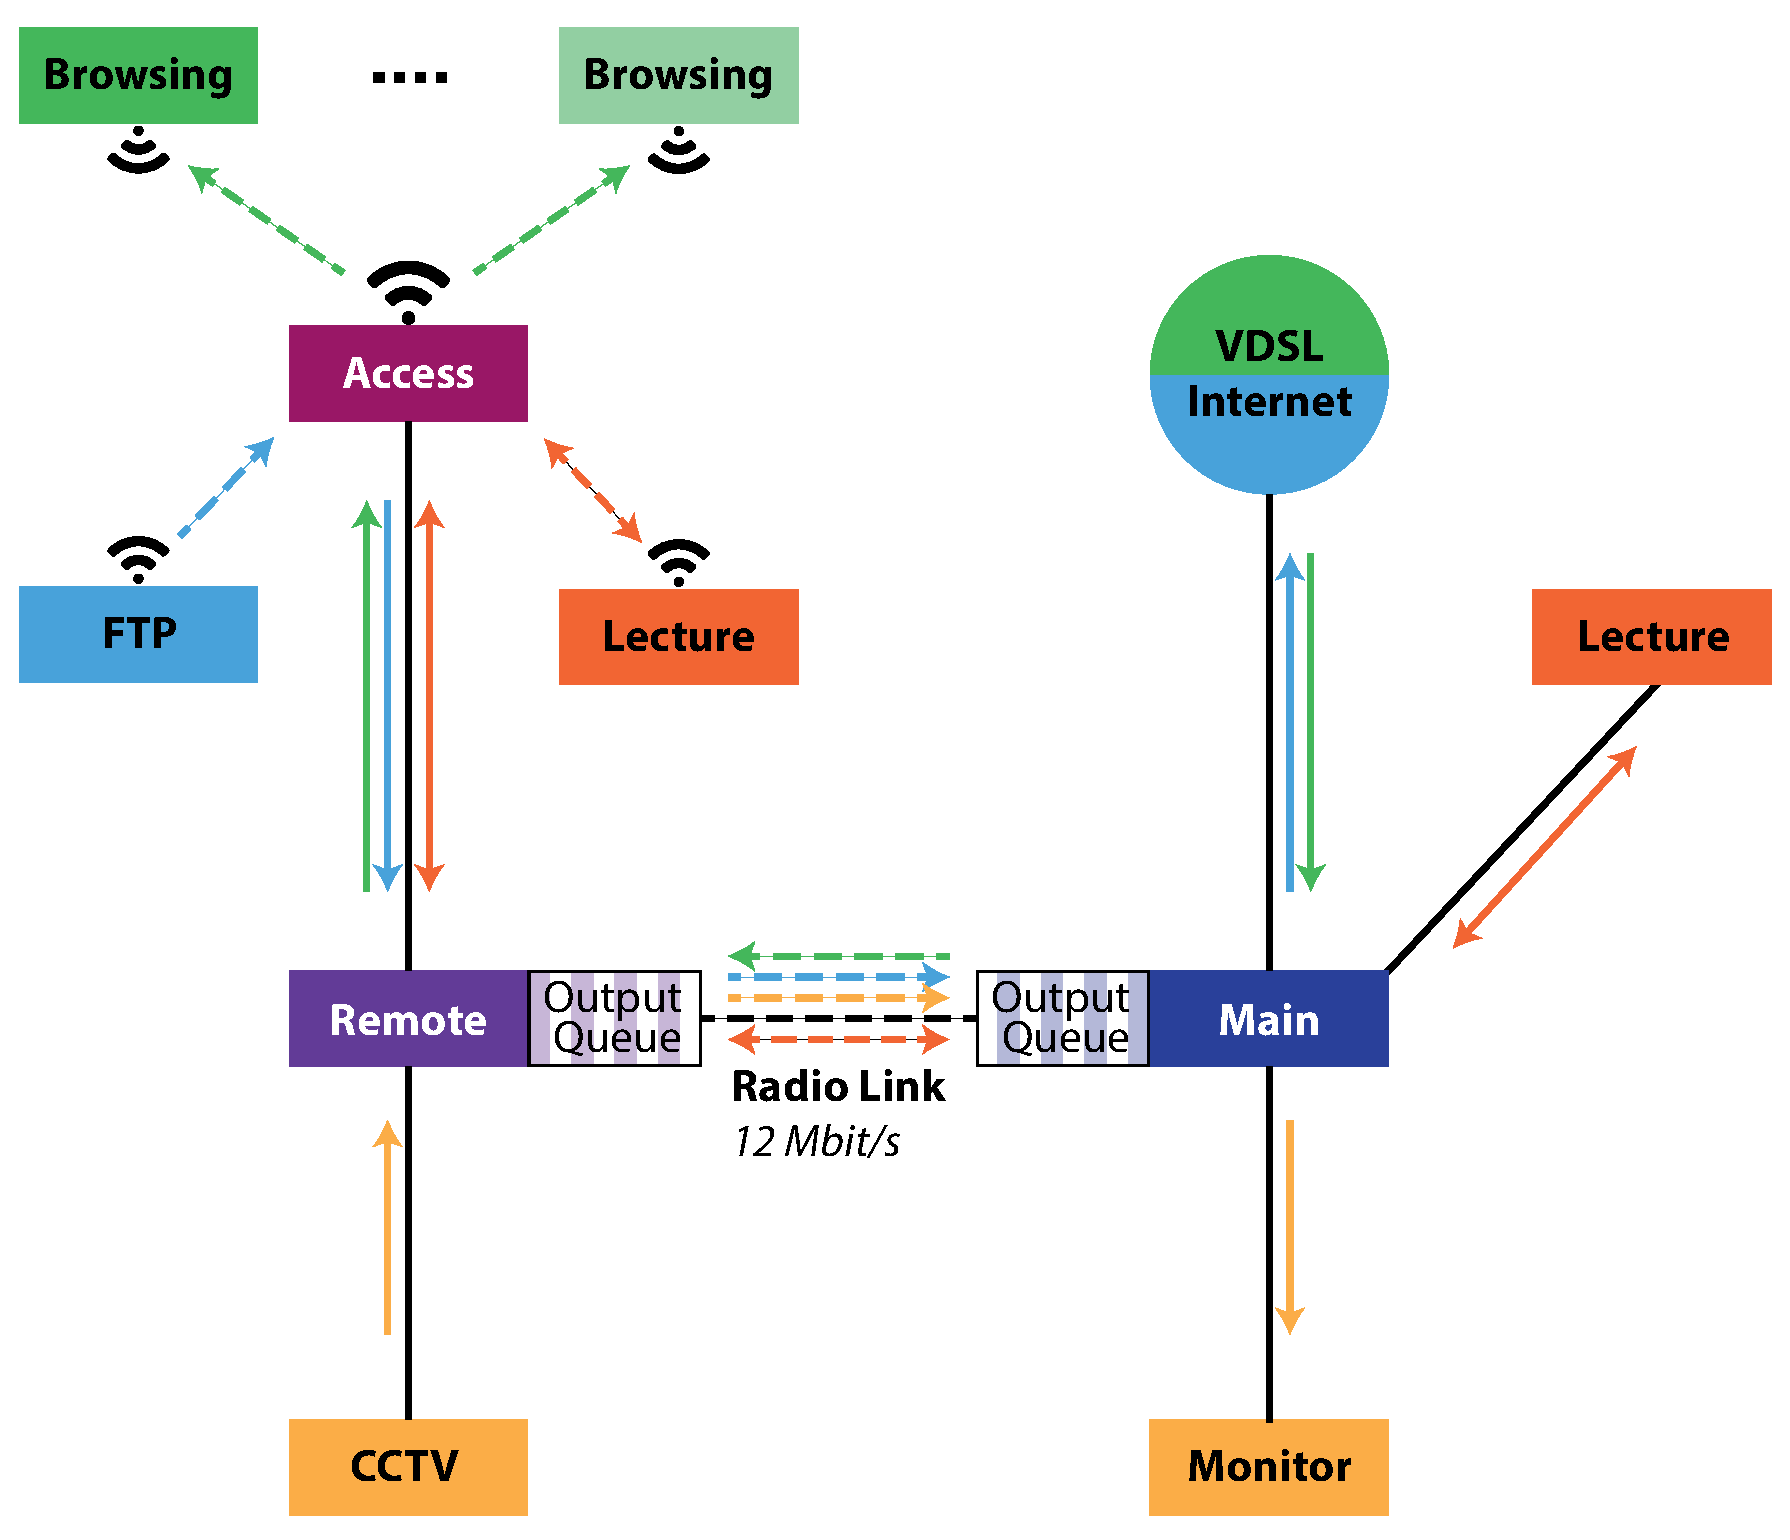
\includegraphics[width=0.9\textwidth]{graphics-03.eps}
    \label{fig:network}
    \caption{University Network}
\end{figure}

\section{General Description of the Network's Main Components}
By Nina Piontek.\\

The network core is a set up with 2 Routers, Main Router and Remote Router, connected with a Point-to-Point Link. 
Towards the Main Router the Porters Office' Computer and the Computer of the Professor giving the remote Lecture are connected.
The Main Router is the Gateway for the shared Internet Connection of the University.

Towards the Remote Router the Access Point for WLAN and the Security Camera are connected.
The Access Point provides Wireless Lan for Students at Channel 4. The Computer for the Video Lecture at Channel 4 
is connected via WLAN as well.



\section{Network Services and Requirements}
By Nina Piontek.\\

In this set up the Network performance regarding the Video Lecture is evaluated with the following Services in
use:\\
\begin{enumerate}
 \item WLAN for Webbrowsing
 \item FTP Service for Uploading a file to a Server in the Internet (used by one Student) 
 \item Video Lecture streamed in both directions from the Main Campus to Channel 4
 \item Security Camera streaming from Channel 4 to the Porters Office  at the Main Campus
\end{enumerate}

The network should provide a certain Quality of Service for the Video Lecture and the Security Camera.
The Criteria are:\\
\begin{enumerate}
 \item The Video Data should not take more than 100ms to be delivered to the destination in both directions.
 \item There should only be a loss of data at most of 5$ \% $
\end{enumerate}

\chapter{Network Modeling}
\section{General Assumptions on the Model}
By Nina Piontek.\\

Since the overall Goal is to evaluate the network performance regarding the Qos during the Video Lecture, we will assume an assessment period
of around 90 minutes. The WLAN at Channel 4 will in general be used by the Students, which surf the Web during the Video Lecture and the Student 
who uploads a file. Optional the Camera will be turned on or switched off to evaluate the networks behavior with and without the additional
traffic load.
\subsection{HTTP Traffic}
\label{chapter_http_traffic}
By Daniel Plöger.\\

In order to model the student web browsing behavior in 
a meaningful way, captured browsing statistics have been provided by the computer center in a trace file. 
This chapter shortly explains the statistical behavior behind the given HTTP 
requests and responses. The response sample traces (download statistics) are widely 
distributed in the range of less than 500 Bytes up to more than 4 Mbyte 
(see figure \ref{fig:trace} top).
\begin{figure}[!ht]
  \centering
    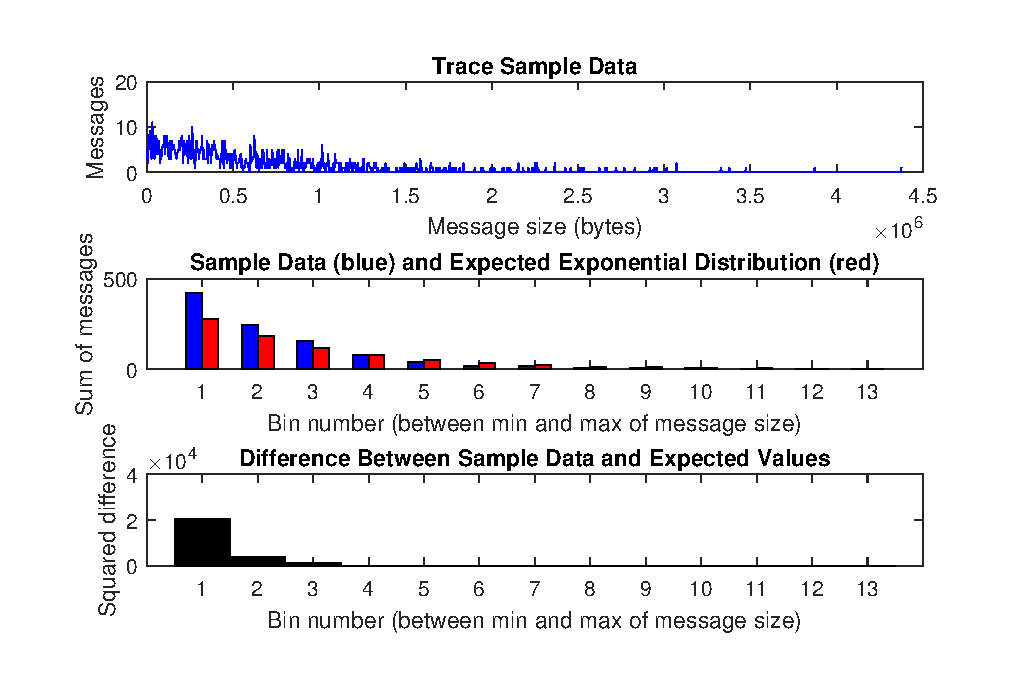
\includegraphics[width=0.9\textwidth]{trace_distribution.eps}
    \label{fig:trace}
    \caption{HTTP Traffic Analysis}
\end{figure}

Distribution fitting analysis shows that the statistical behavior if
 partitioned in a smaller number of bins roughly behaves like a negative 
exponential distribution with a mean value of 0.789 Mbyte (see figure \ref{fig:trace} center) \cite{goodness_of_fit}. 
The phrase "roughly" means that while the statistical goodness of fit tests accepts
 this distribution, the actual data has an overweight of small messages compared to
 the expected values (see figure \ref{fig:trace} bottom). An exponential distribution with the
 mean of 0.789 Mbyte is used in this report for simulation nonetheless. 
This is a conservative approach and guarantees an upper bound in the distribution:
 if the actual browsing behavior uses smaller HTTP responses with a slightly higher
 probability, the QoS assumptions from the following chapters are going to be met 
in practice as well.
\section{Network Behavior  Expectations without CCTV camera}
By Nina Piontek.\\

\begin{minipage}[t]{0.5\textwidth}
\begin{tabular}{|l|l|l|l|l|}
\cline{1-4}
 Link & Data Rate  & Downlink  & Uplink  \\ \cline{1-4}
 WLAN & 54Mbit/s  & HTTP, Video Lecture & FTP,Video Lecture \\ \cline{1-4}
 Access Point $\leftrightarrow$ Remote Router & 100Mbit/s  &HTTP, Video Lecture& FTP  \\ \cline{1-4}
 Camera $\leftrightarrow$ Remote Router & 100Mbit/s  & - & Camera\\ \cline{1-4}
 Remote Router$\leftrightarrow$Main Router&12 Mbit/s&HTTP,Video Lecture& FTP, \\ 
 & & & Video Lecture,Camera \\ \cline{1-4}
 Main Router$\leftrightarrow $ Porters Office &Ideal Connection &Camera& - \\ \cline{1-4}
 Main Router$\leftrightarrow $ Professor & -  &Video Lecture&Video Lecture \\ \cline{1-4}
 Main Router$\leftrightarrow $ Internet &100Mbit/s &HTTP& FTP \\ \cline{1-4}
\end{tabular}
\end{minipage}
\section{Network Behavior Expectations with CCTV camera turned on}
\label{chapter_expectations}
By Daniel Plöger.\\

The point-to-point radio link between remote and main router has a full duplex data rate of 12 Mbit/s and by this is the weakest single link within the proposed network. All other connection speeds are multiples of this data rate. Since all data has to pass this link, for this theoretical behavior analysis it is considered to be the network bottleneck.
\begin{figure}[!ht]
  \centering
    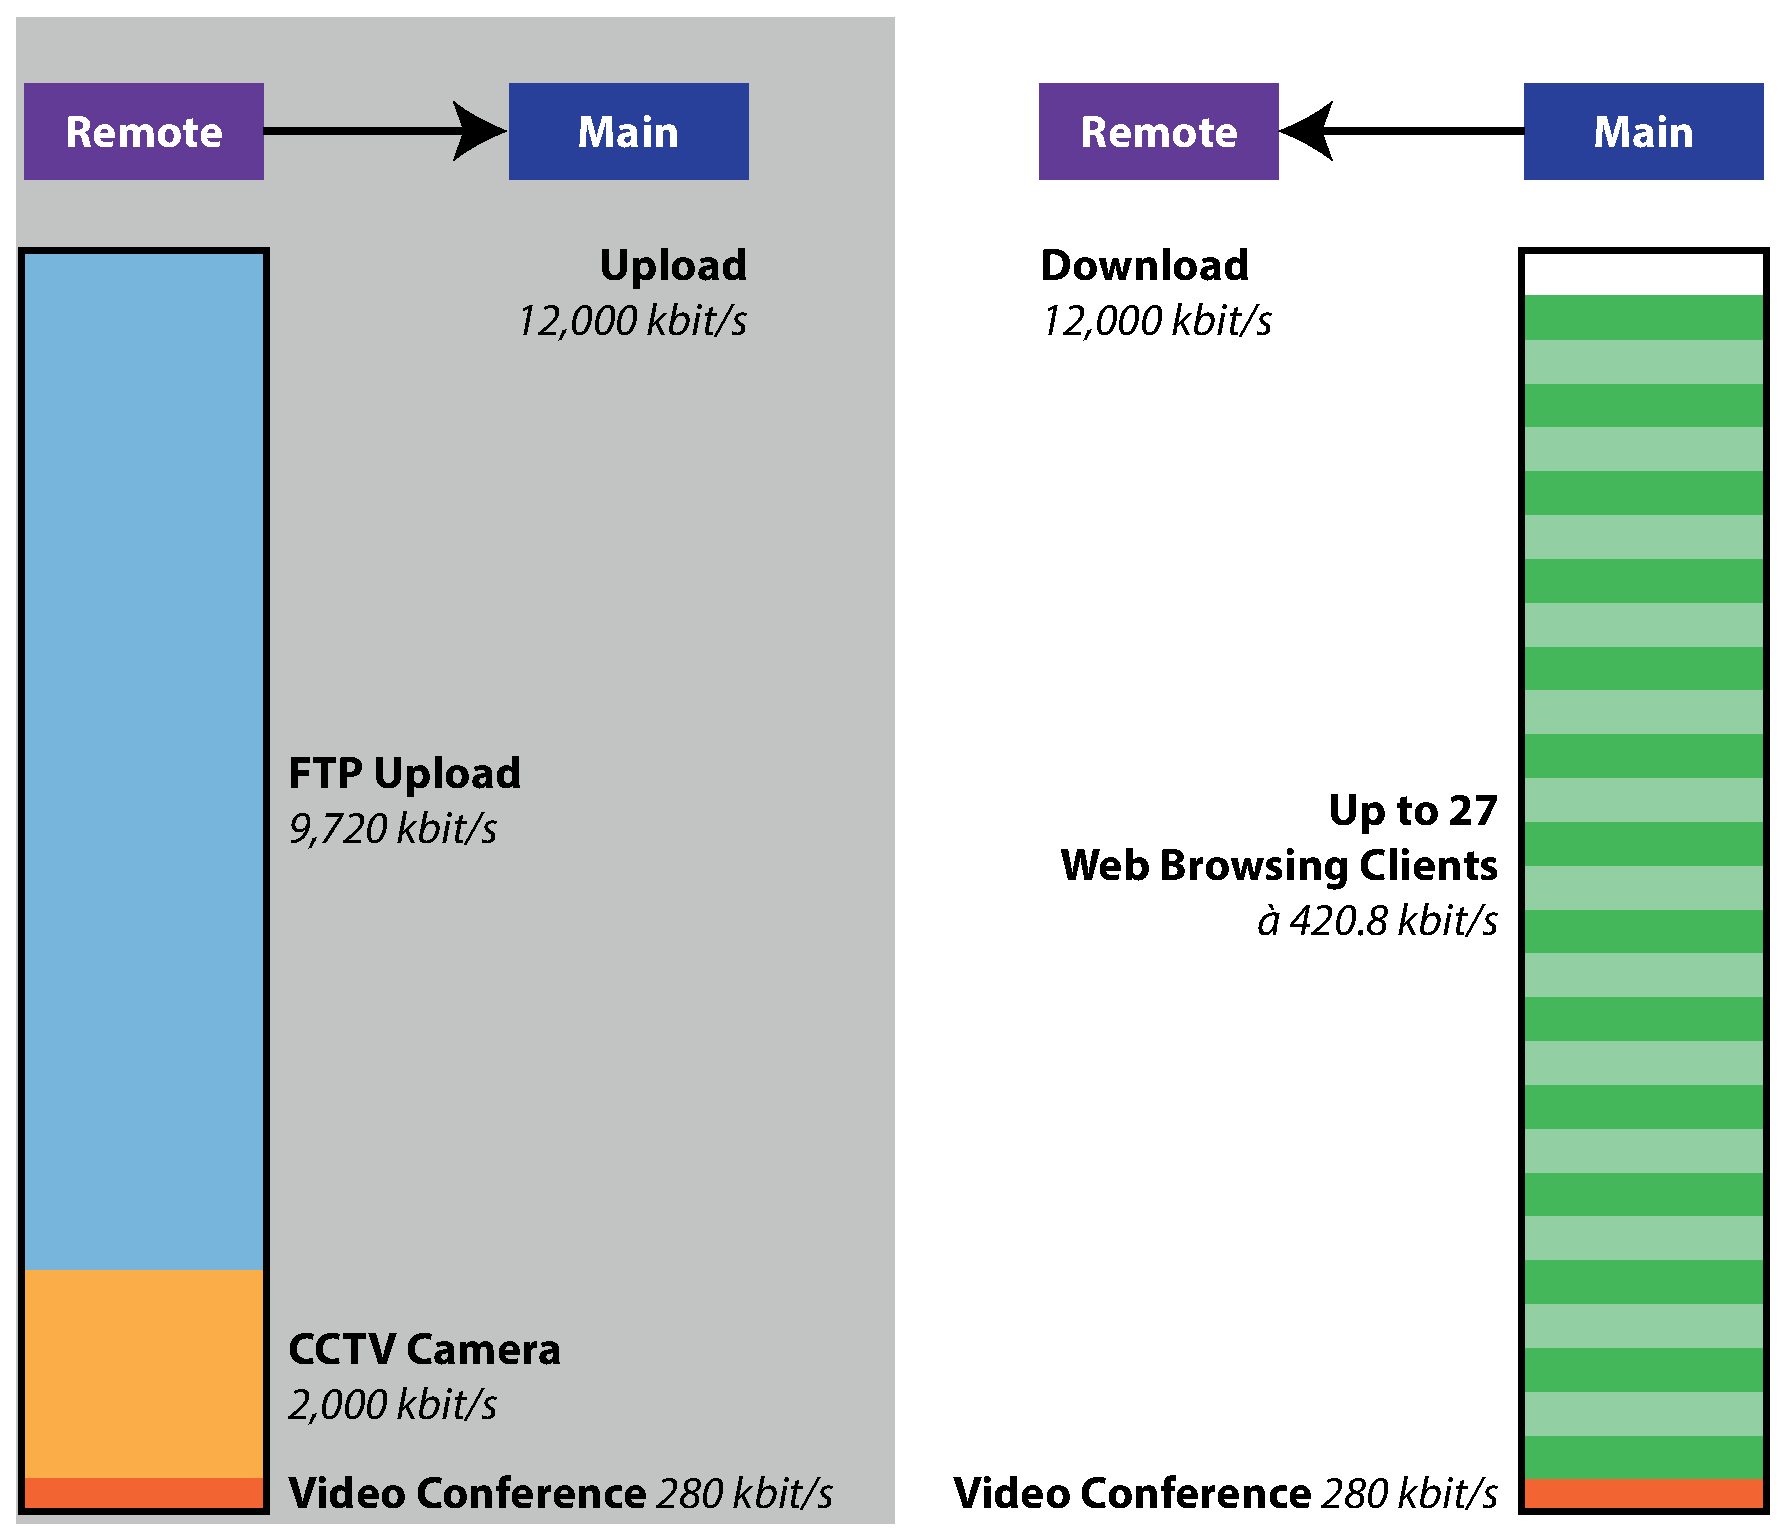
\includegraphics[width=0.9\textwidth]{graphics-01.eps}
    \label{fig:radio_link_theory_on}
    \caption{Max. Possible Utilization of the Radio Link With the CCTV Camera Streaming}
\end{figure}

The network contains several applications which have their main impact either on the download connection from the main router to the remote router, or on the upload connection in the other direction. The respective opposite direction of an application may be neglected, since it mainly consists of very small messages for connection management or empty network packets. For this reason, theoretical down- and upload utilization is examined independently from each other in this chapter. 

The only exception is the video conference, which utilizes both, up- and download equally. The video stream consumes 280 kbit/s for transmission of 1388 Bytes of payload plus 12 Byte RTP protocol headers. It does this every 40 ms and in both directions.

\subsection{Upload Connection, Remote to Main Router}
Aside from the video conference which uses 280 kbit/s, two more applications make use of the upload direction. Firstly, the CCTV camera sends 10 kByte every 40 ms, which adds up to 2,000 kbit/s. The second application is the FTP upload. It tries to maximize network utilization and should therefore consume the biggest part of the remaining 9,720 kbit/s of the total 12,000 kbit/s data rate (see figure \ref{fig:radio_link_theory_on} left).

\subsection{Download Connection, Main to Remote Router}
Other than the video conference, the only application which makes use of the download direction is the web browsing. As stated before, web browsing is modeled as the download of files with an exponentially distributed size with a mean of 0.789 Mbyte (see chapter \ref{chapter_http_traffic}). The client's assumption states that a web browsing user waits a certain time before he downloads the next file. The waiting time is assumed to be exponentially distributed with a mean of 15 seconds. This leads to an expected average data rate of 420.8 kbit/s per user. Therefore, if all users download in a well-distributed way, up to 27 users are able to browse simultaneously via the network connection (see figure \ref{fig:radio_link_theory_on} right).

\subsection{Conclusion}
For a fully-functional network that guarantees both the CCTV camera and the video lecture conference to satisfy all quality of service requirements, the proposed network is not able to allow for many additional applications or users. In theory, a classroom in the given size could host up to 800 tightly seated students for lecture \cite{sitzkultur}. The expected behavior suggests that in theory up to 27 of them are able to browse the web at the same time without restricting the video streams. 

In practice however the network is expected to permit even less simultaneous users. This is due to the nature of HTTP requests and responses: the requested data is not perfectly distributed over time. Instead, high peaks of transmitted data occur at certain points in time, alternated with moments of complete silence. The video streams on the other hand are expected to transmit reliable at any point in time.

Meanwhile, the FTP upload and the CCTV camera stream is expected to be mostly independent of the number of web clients. The main transmission direction of these applications is upwards from the remote site to the main campus, opposite to the web browsing downloads. With higher numbers of web clients, the uploads are expected to slow down very little only due to the rising number of session handling messages from the underlying protocols.

\chapter{Evaluation without Camera}
By Nina Piontek.\\

Since the default configuration for the Links is full-duplex, the performance of the Uplink and the Downlink is evaluated independently.

When the Camera is turned off, the Point-to-Point Link to the Main Campus is shared between the FTP Upload and the Video Lecture (Video Conference).
Since the Video Conference is sending with a constant Data Rate of 280kbit/s, the remaining 
11,72 Mbit/s can be used by the FTP Upload.
\begin{figure}[!ht]
  \centering
    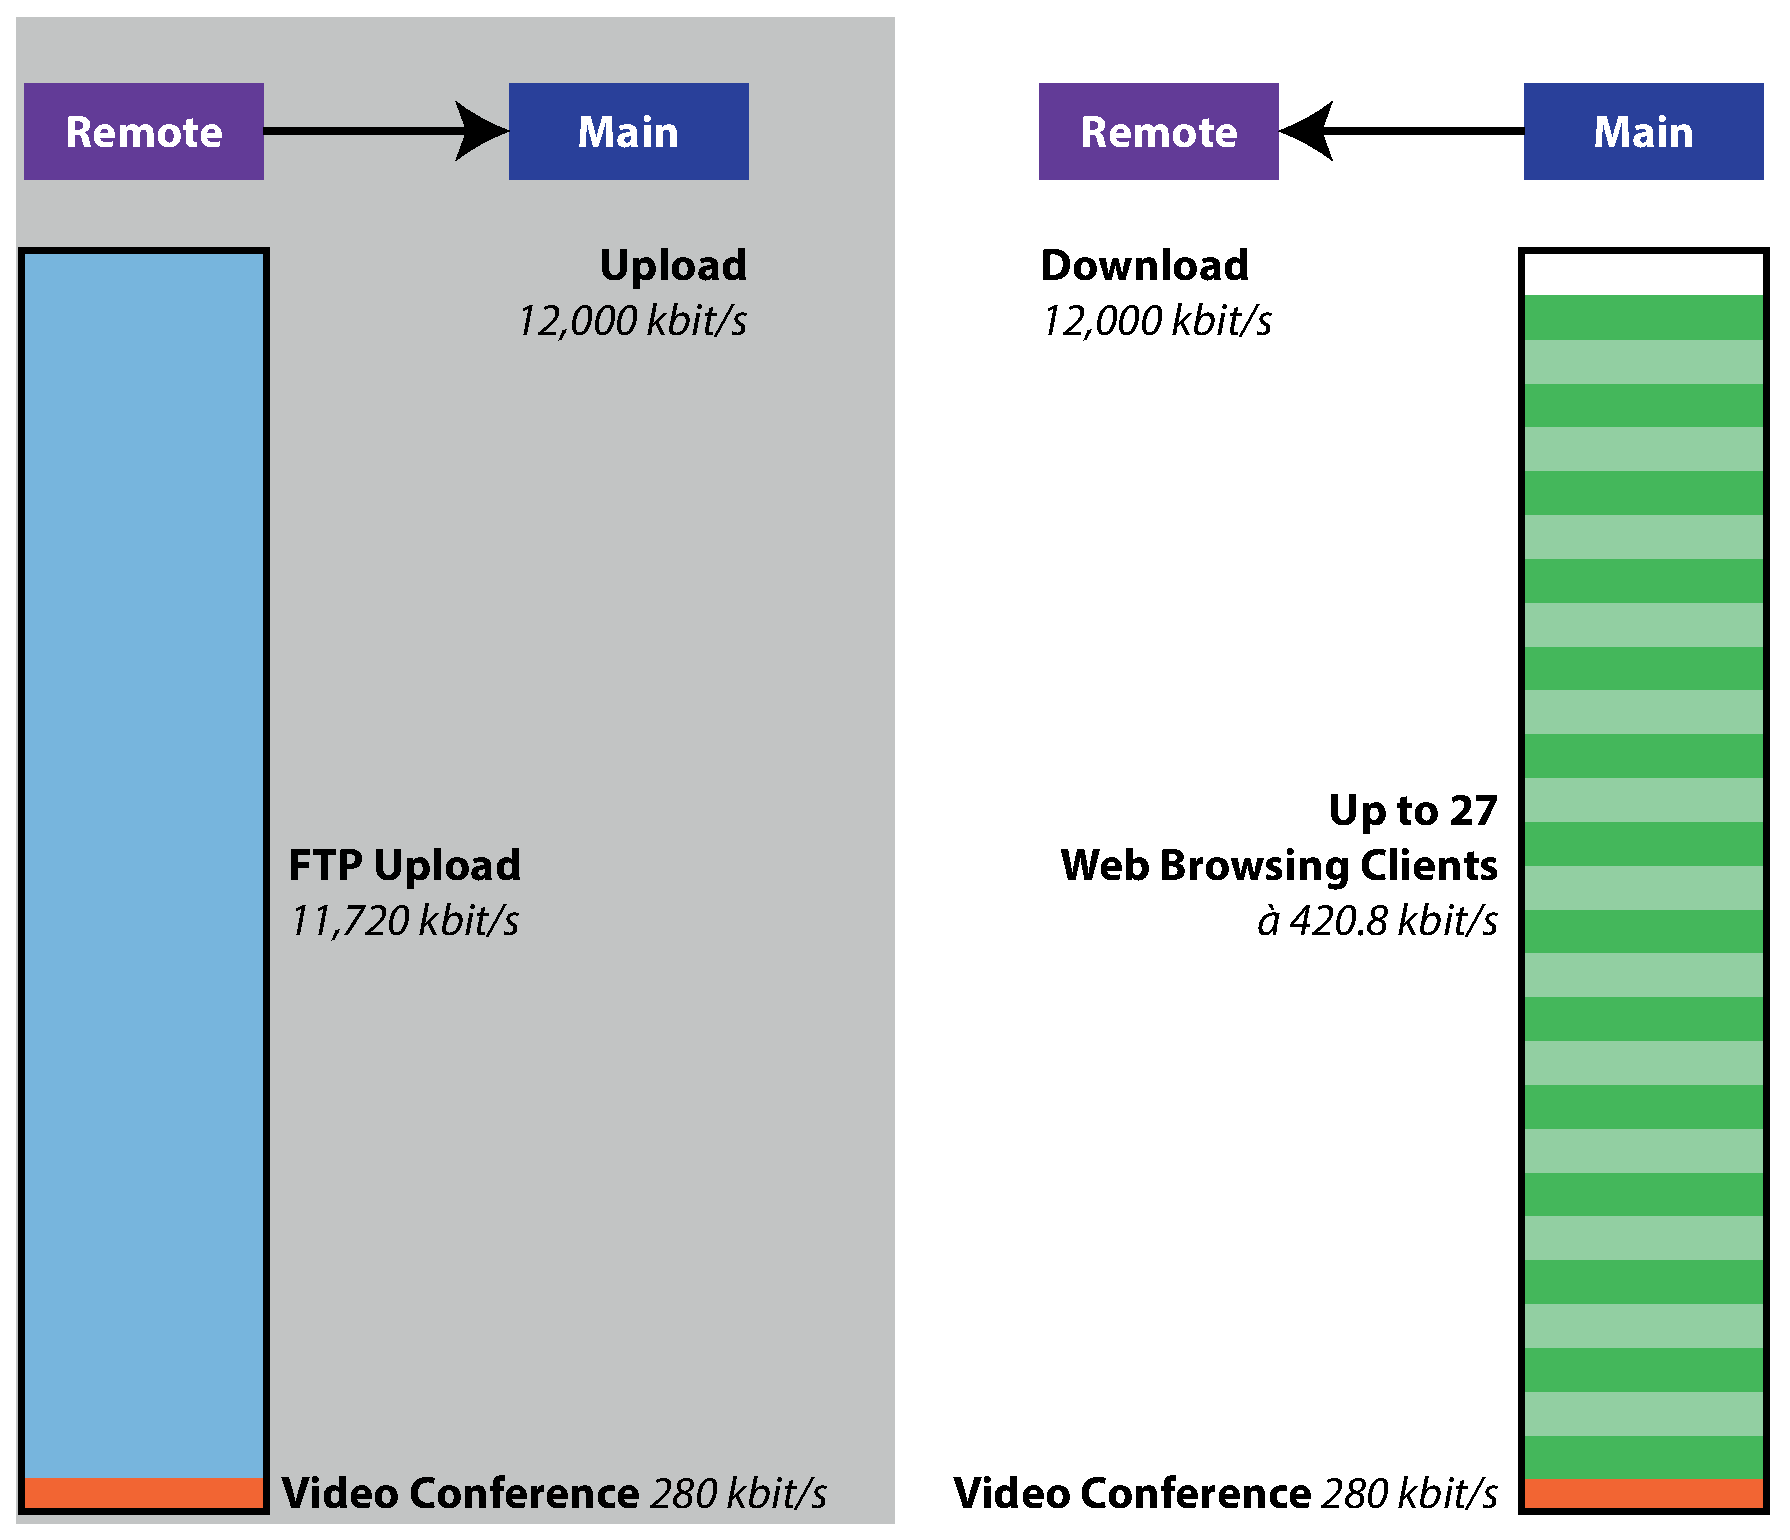
\includegraphics[width=0.9\textwidth]{graphics-02.eps}
    \label{fig:g2}
    \caption{Utilization of the Radio Link without the Security Camera streaming}
\end{figure}

On the Downlink the Data Rate of 12Mbit/s is shared between the Students browsing the Web (HTTP Service) and the Video Lecture (Video Conference).
Since the Downlink is utilized by the Video Lecture by 280kbit/s , the remaining 11,7Mbit/s 
can be theoretically used by the HTTP Service.

\section{Simulation Results}

Text.




\chapter{Evaluation With Camera Turned On}
By Daniel Plöger.\\

In order to assess the proposed network, the behavior was simulated and will be evaluated in this chapter. The evaluation is divided into the sections \textit{loss rates and delays analysis}, \textit{HTTP data rates}, \textit{FTP data rate}, and \textit{main bottlenecks}. In each section, the results are examined with regards to the number of HTTP users that are web browsing simultaneously and compared to the expected behavior from chapter \ref{chapter_expectations}.

\section{Loss Rates and Delays Analysis}

The conference stream of the video lecture is analyzed in both directions. In the upload from the remote classroom to the professor's laptop, the video quality-of-service is not becoming worse with more number of users. The loss rate is  negligible the whole time. This was predicted in the expected performance, since the direction of the video upstream is opposite to the HTTP download.

\begin{figure}[!ht]
  \centering
    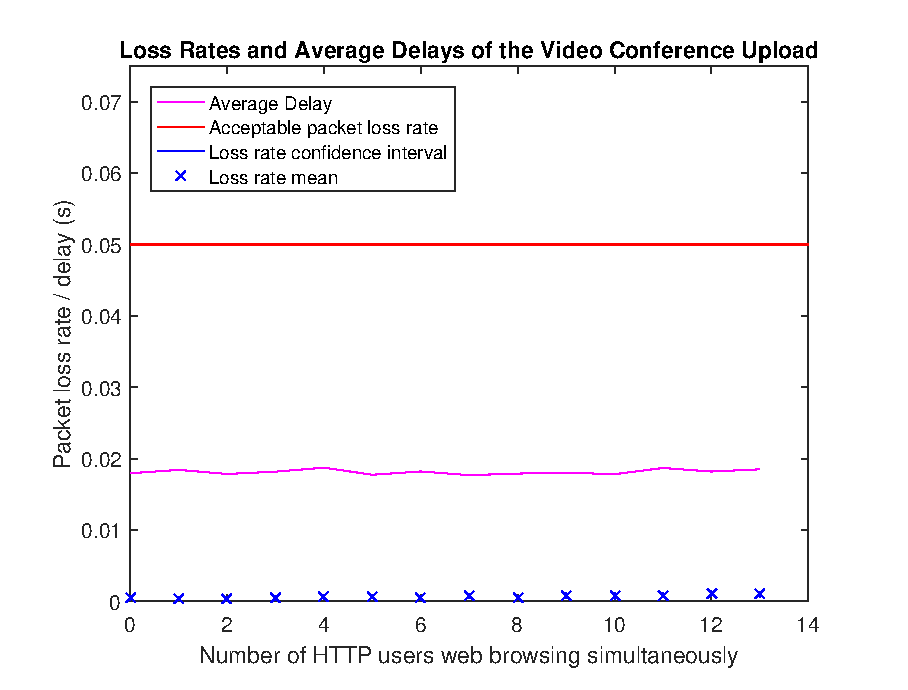
\includegraphics[width=0.9\textwidth]{on_loss_conf_upload.eps}
    \label{fig:on_loss_conf_upload}
    \caption{TODO}
\end{figure}

\begin{figure}[!ht]
  \centering
    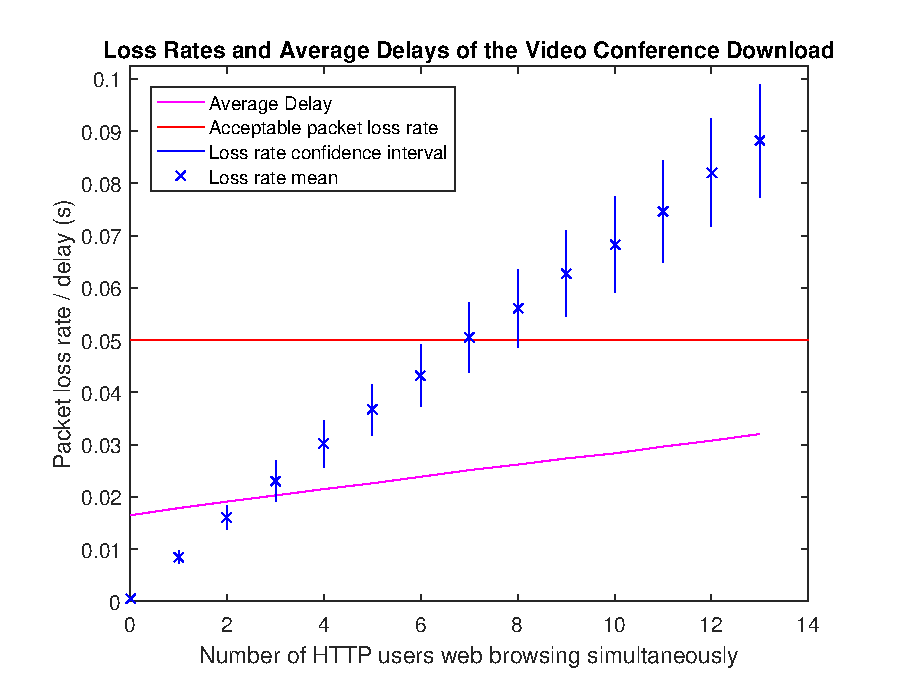
\includegraphics[width=0.9\textwidth]{on_loss_conf_download.eps}
    \label{fig:on_loss_conf_download}
    \caption{TODO}
\end{figure}

\begin{figure}[!ht]
  \centering
    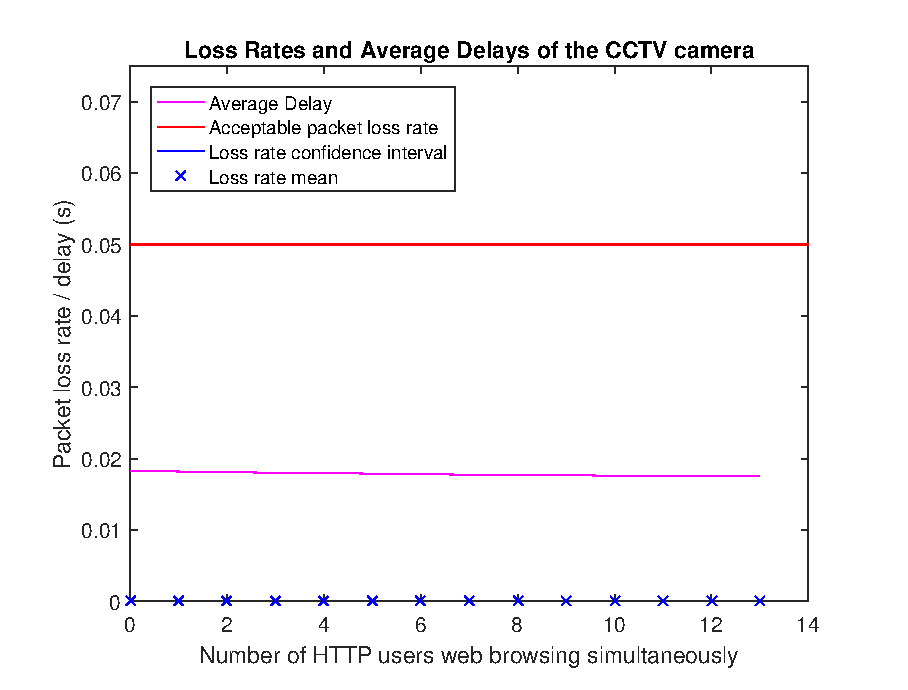
\includegraphics[width=0.9\textwidth]{on_loss_cctv.eps}
    \label{fig:on_loss_cctv}
    \caption{TODO}
\end{figure}


\section{TODO}
\begin{figure}[!ht]
  \centering
    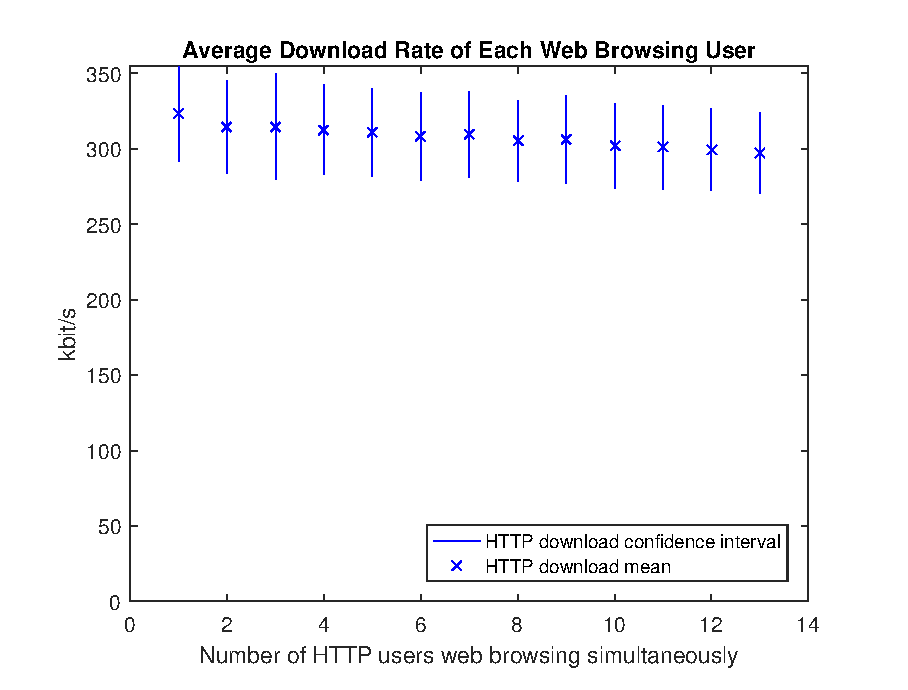
\includegraphics[width=0.9\textwidth]{on_http_download.eps}
    \label{fig:on_http_download}
    \caption{TODO}
\end{figure}

\begin{figure}[!ht]
  \centering
    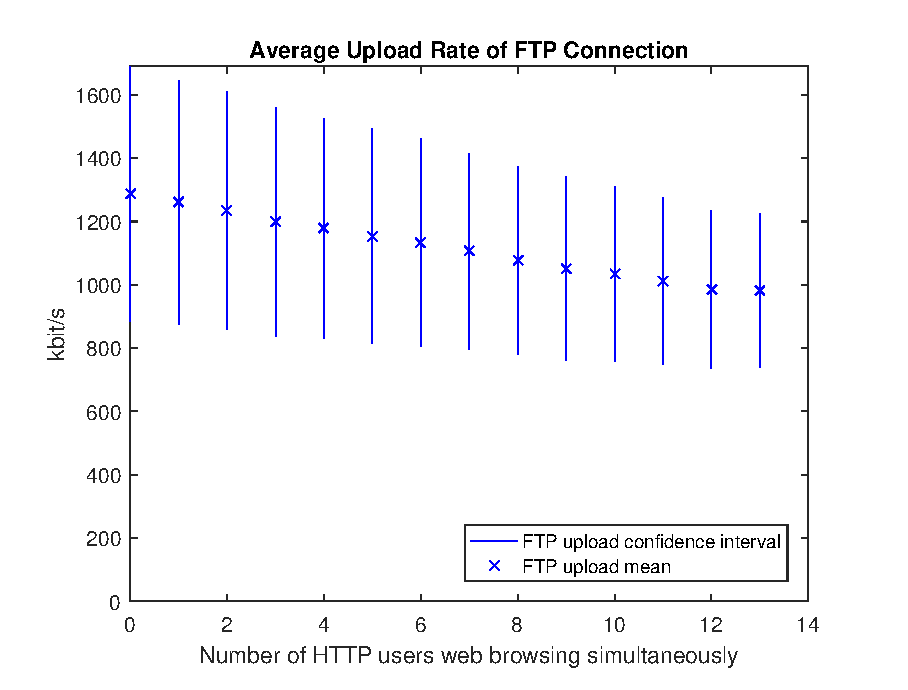
\includegraphics[width=0.9\textwidth]{on_ftp_upload.eps}
    \label{fig:on_ftp_upload}
    \caption{TODO}
\end{figure}


\begin{figure}[!ht]
  \centering
    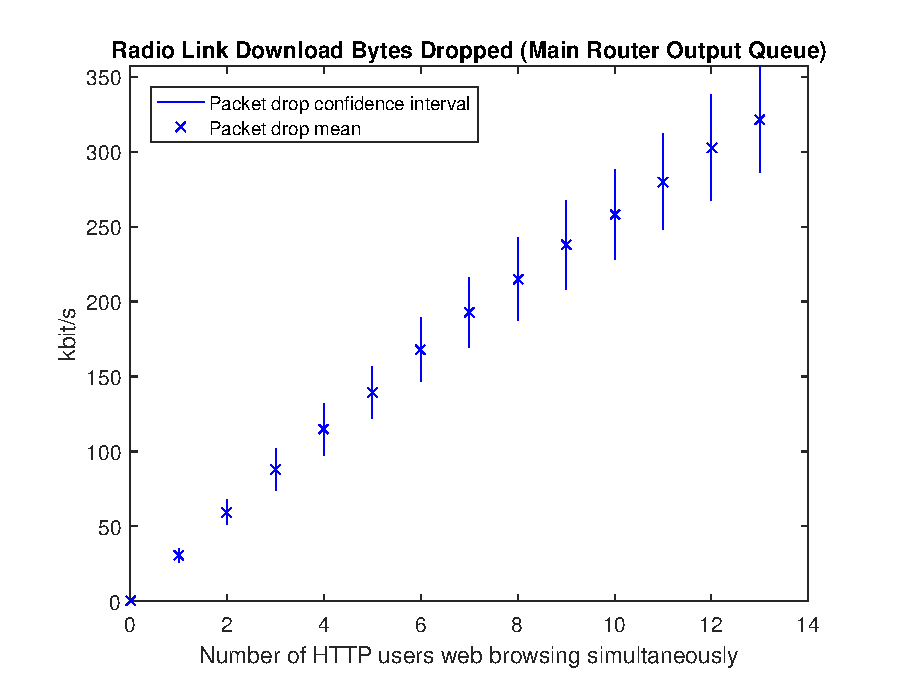
\includegraphics[width=0.9\textwidth]{on_main_router_drops.eps}
    \label{fig:on_main_router_drops}
    \caption{TODO}
\end{figure}

\begin{figure}[!ht]
  \centering
    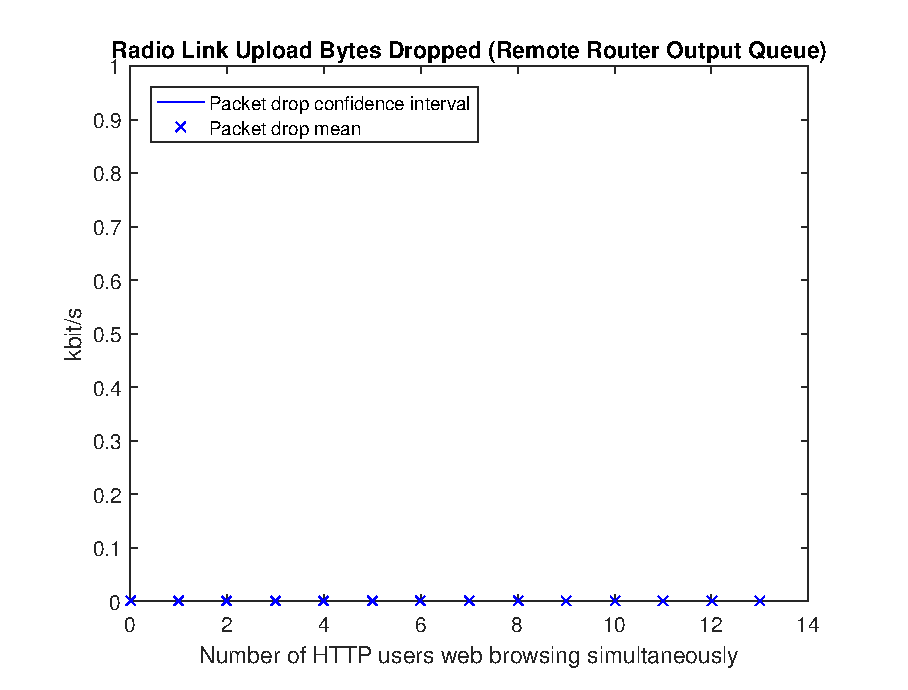
\includegraphics[width=0.9\textwidth]{on_remote_router_drops.eps}
    \label{fig:on_remote_router_drops}
    \caption{TODO}
\end{figure}
         

\chapter{Conclusion and Suggestions}

Text.

	\bibliographystyle{plain}
	\bibliography{bibliography}
\end{document} 